\documentclass[a4paper,UTF8]{article}
\usepackage{ctex}
\usepackage[margin=1.25in]{geometry}
\usepackage{color}
\usepackage{graphicx}
\usepackage{amssymb}
\usepackage{amsmath}
\usepackage{amsthm}
\usepackage{enumerate}
\usepackage{bm}
\usepackage{hyperref}
\usepackage{pgfplots}
\usepackage{epsfig}
\usepackage{color}
\usepackage{tcolorbox}
\usepackage{mdframed}
\usepackage{lipsum}
\usepackage{framed}
\usepackage{setspace}
\usepackage{float} %设置图片浮动位置的宏包

\newmdtheoremenv{thm-box}{myThm}
\newmdtheoremenv{prop-box}{Proposition}
\newmdtheoremenv{def-box}{定义}

\setlength{\evensidemargin}{.25in}
\setlength{\textwidth}{6in}
\setlength{\topmargin}{-0.5in}
\setlength{\topmargin}{-0.5in}
% \setlength{\textheight}{9.5in}
%%%%%%%%%%%%%%%%%%此处用于设置页眉页脚%%%%%%%%%%%%%%%%%%
\usepackage{fancyhdr}                                
\usepackage{lastpage}                                           
\usepackage{layout}                                             
\footskip = 10pt 
\pagestyle{fancy}                    % 设置页眉                 
\lhead{2022年秋季}                    
\chead{数字信号处理}                                                
% \rhead{第\thepage/\pageref{LastPage}页} 
\rhead{作业一}                                                                                               
\cfoot{\thepage}                                                
\renewcommand{\headrulewidth}{1pt}  			%页眉线宽,设为0可以去页眉线
\setlength{\skip\footins}{0.5cm}    			%脚注与正文的距离           
\renewcommand{\footrulewidth}{0pt}  			%页脚线宽,设为0可以去页脚线

\makeatletter 									%设置双线页眉                                        
\def\headrule{{\if@fancyplain\let\headrulewidth\plainheadrulewidth\fi%
\hrule\@height 1.0pt \@width\headwidth\vskip1pt	%上面线为1pt粗  
\hrule\@height 0.5pt\@width\headwidth  			%下面0.5pt粗            
\vskip-2\headrulewidth\vskip-1pt}      			%两条线的距离1pt        
 \vspace{6mm}}     								%双线与下面正文之间的垂直间距              
\makeatother  

%%%%%%%%%%%%%%%%%%%%%%%%%%%%%%%%%%%%%%%%%%%%%%
\numberwithin{equation}{section}
%\usepackage[thmmarks, amsmath, thref]{ntheorem}
\newtheorem{myThm}{myThm}
\newtheorem*{myDef}{Definition}
\newtheorem*{mySol}{Solution}
\newtheorem*{myProof}{Proof}
\newtheorem*{myRemark}{备注}
\renewcommand{\tilde}{\widetilde}
\renewcommand{\hat}{\widehat}
\newcommand{\indep}{\rotatebox[origin=c]{90}{$\models$}}
\newcommand*\diff{\mathop{}\!\mathrm{d}}

\usepackage{multirow}

%--

%--
\begin{document}

\title{数字信号处理\\
作业一}
\author{方盛俊\, 201300035} 
\maketitle
%%%%%%%% 注意: 使用XeLatex 编译可能会报错,请使用 pdfLaTex 编译 %%%%%%%

\section*{作业提交注意事项}
\begin{tcolorbox}
\begin{enumerate}
  \item[(1)] 本次作业提交截止时间为~\textcolor{red}{\textbf{2022/11/27  23:59:59}},截止时间后不再接收作业,本次作业记零分;
  \item[(2)] 作业提交方式:使用此~LaTex~模板书写解答,只需提交编译生成的~pdf~文件,将~pdf~文件以ftp方式上传,账号为dsp2022,密码为12345asd!@。请远程连接www.lamda.nju.edu.cn,提交到/D:/courses/DSP2022/HW/HW1路径下。
  \item[(3)] 文件命名方式:学号-姓名-作业号-v版本号, 例~ MG1900000-张三-1-v1;如果需要更改已提交的解答,请在截止时间之前提交新版本的解答,并将版本号加一;
  \item[(4)] 未按照要求提交作业,或~pdf~命名方式不正确,将会被扣除部分作业分数。

\end{enumerate}
\end{tcolorbox}


\newpage
\section{[20pts] 信号的周期性}
判断下列信号的周期性,并回答\textbf{是}、\textbf{否}或\textbf{无法判断}。如果是周期信号,请给出其最小正周期。
\begin{enumerate}[(1)]
	\item $x(t)=\sin^2t+\cos\pi t$
	\item $x(t)=(\sin2t+\cos t)^2$
	\item $x(t)=\displaystyle\frac{\cos2t+1+\sin t+\sin2t+\sin3t}{\cos t}$
	\item $x(t)=\sin et+\cos\pi t$
	\item $x(n)=\sin 2kn+\cos 3kn$, $k$为某一正实数。
\end{enumerate}

\begin{framed}
\begin{spacing}{1.5}
    \begin{itemize}
      \item (1)
      
      $\displaystyle x(t) = \sin ^{2}t + \cos \pi t = \frac{1}{2}-\frac{1}{2}\cos 2t + \cos \pi t$
      
      其中 $\cos 2t$ 周期为 $\displaystyle T_1 = \frac{2\pi}{2} = \pi$, $\cos \pi t$ 的周期为 $\displaystyle T_2 = \frac{2\pi}{\pi} = 2$.
      
      由于 $\displaystyle \frac{T_1}{T_2} = \frac{\pi}{2}$ 为无理数, 因此 $x(t)$ 不是周期信号.
      
      \item (2)
      
      $
      \begin{aligned}
      x(t) &= (\sin 2t + \cos t)^{2} \\
      &= \sin^{2} 2t + 2\sin 2t\cos t + \cos^{2} t \\
      &= \frac{1}{2}-\frac{1}{2}\cos 4t + (\sin (2t+t)+\sin (2t-t)) + \frac{1}{2}\cos 2t+\frac{1}{2} \\
      &= -\frac{1}{2}\cos 4t + \sin 3 t + \frac{1}{2}\cos 2t+\sin t+1 \\
      \end{aligned}
      $
      
      由于 $\cos 4t, \sin 3t, \cos 2t, \sin t$ 的周期分别为 $\displaystyle \frac{\pi}{2}, \frac{2\pi}{3}, \pi, 2\pi$.
      
      它们两两间的周期之比为有理数, 因此 $x(t)$ 为周期信号, 周期为它们的最小公倍数 $\displaystyle 2\pi$.
      
      \item (3)
      
      $
      \begin{aligned}
      x(t) &= \frac{\cos 2t + 1 + \sin t + \sin 2t + \sin 3t}{\cos t} \\
      &= \frac{2\cos^{2} t + \sin t + 2\sin t\cos t + 3\sin t - 4\sin^{3} t}{\cos t} \\
      &= \frac{2\cos^{2} t + 4\sin t + 2\sin t\cos t - 4\sin t(1 - \cos^{2} t)}{\cos t} \\
      &= \frac{2\cos^{2} t + 2\sin t\cos t + 4\sin t\cos^{2} t}{\cos t} \\
      &= \frac{2\cos^{2} t + 2\sin t\cos t + 2\sin 2t\cos t}{\cos t} \\
      &= 2\cos t + 2\sin t + 2\sin 2t \\
      \end{aligned}
      $
      
      其中 $\cos t, \sin t, \sin 2t$ 的周期分别为 $2\pi, 2\pi, \pi$.
      
      它们两两间的周期之比为有理数, 因此 $x(t)$ 为周期信号, 周期为它们的最小公倍数 $\displaystyle 2\pi$.
      
      \item (4)
      
      $x(t) = \sin et + \cos \pi t$

      其中 $\sin et, \cos \pi t$ 的周期分别为 $\displaystyle \frac{2\pi}{e}, 2$.
      
      由于 $\displaystyle \frac{T_1}{T_2} = \frac{\pi}{e}$ 不清楚是有理数还是无理数, 因此无法判定 $x(n)$ 的周期性.
      
      \item (5)
      
      $x(n) = \sin 2kn + \cos 3kn$

      若令 $\sin 2k(n+N) = \sin 2kn$
      
      则我们可知 $2kN = 2\pi m_1$
      
      即 $2kN$ 是 $2\pi$ 的整数倍, 且周期为 $\displaystyle N = \frac{\pi m_1}{k}$
      
      若令 $\cos 3k(n+N) = \cos 3kn$
      
      则我们可知 $3kN = 2\pi m_2$
      
      即 $3kN$ 是 $2\pi$ 的整数倍, 且周期为 $\displaystyle N = \frac{2\pi m_2}{3k}$
      
      如果同时有 $2kN = 2\pi m_1$ 与 $3kN = 2\pi m_2$
      
      则我们两式相减有 $kN = 2\pi(m_2-m_1)$, 即 $kN$ 是 $2\pi$ 的整数倍,
      
      且 $kN$ 是 $2\pi$ 的整数倍也可以推出 $2kN$ 和 $3kN$ 是 $2\pi$ 的整数倍.
      
      若未知 $k$ 为多少, 则无法判定 $x(n)$ 的周期性.
      
      若存在正整数 $N$ 使得其满足 $kN$ 是 $2\pi$ 的整数倍, 则有 $x(n)$ 为周期信号, 且周期为 $\displaystyle N = \frac{2\pi m}{k}$, 其中 $m$ 是使得 $kN=2\pi m$ 成立的最小正整数.
      
      若不存在正整数 $N$ 使得其满足 $kN$ 是 $2\pi$ 的整数倍, 则 $x(n)$ 不是周期信号.
      
    \end{itemize}
\end{spacing}
\end{framed}


\newpage
\section{[22pts] 连续信号的性质与变换}
已知信号
\begin{equation*}
    \begin{aligned}
    x(t)=\left\{
    \begin{aligned}
    & \frac{1}{2}(t+1), && t\in[-1,1]\\
    & 1, && t\in[1,3]\\
    & 0, && other
    \end{aligned}
    \right.
    \end{aligned}
\end{equation*}
\begin{enumerate}[(1)]
	\item 求$x(t)+x(3-\displaystyle\frac{1}{2}t)u(3-t)$的表达式和图像。
	\item 求$x^{\prime}(t)-x^{\prime\prime}(t)$的表达式和图像。(冲激偶函数用$\delta^{\prime}(t)$表示,其图像为原点向y轴正负半轴分别延伸的箭头)
	\item 设$h(t)=\displaystyle\sum^{\infty}_{n=0}\frac{1}{2^n}\left[x(t+4n)+x(t-4n)\right]$, $h(t)$是否为能量信号或功率信号?请说明理由。
\end{enumerate}
	
\begin{framed}
\begin{spacing}{1.5}
    \begin{itemize}
      \item (1)

      \begin{figure}[H]
        \centering
        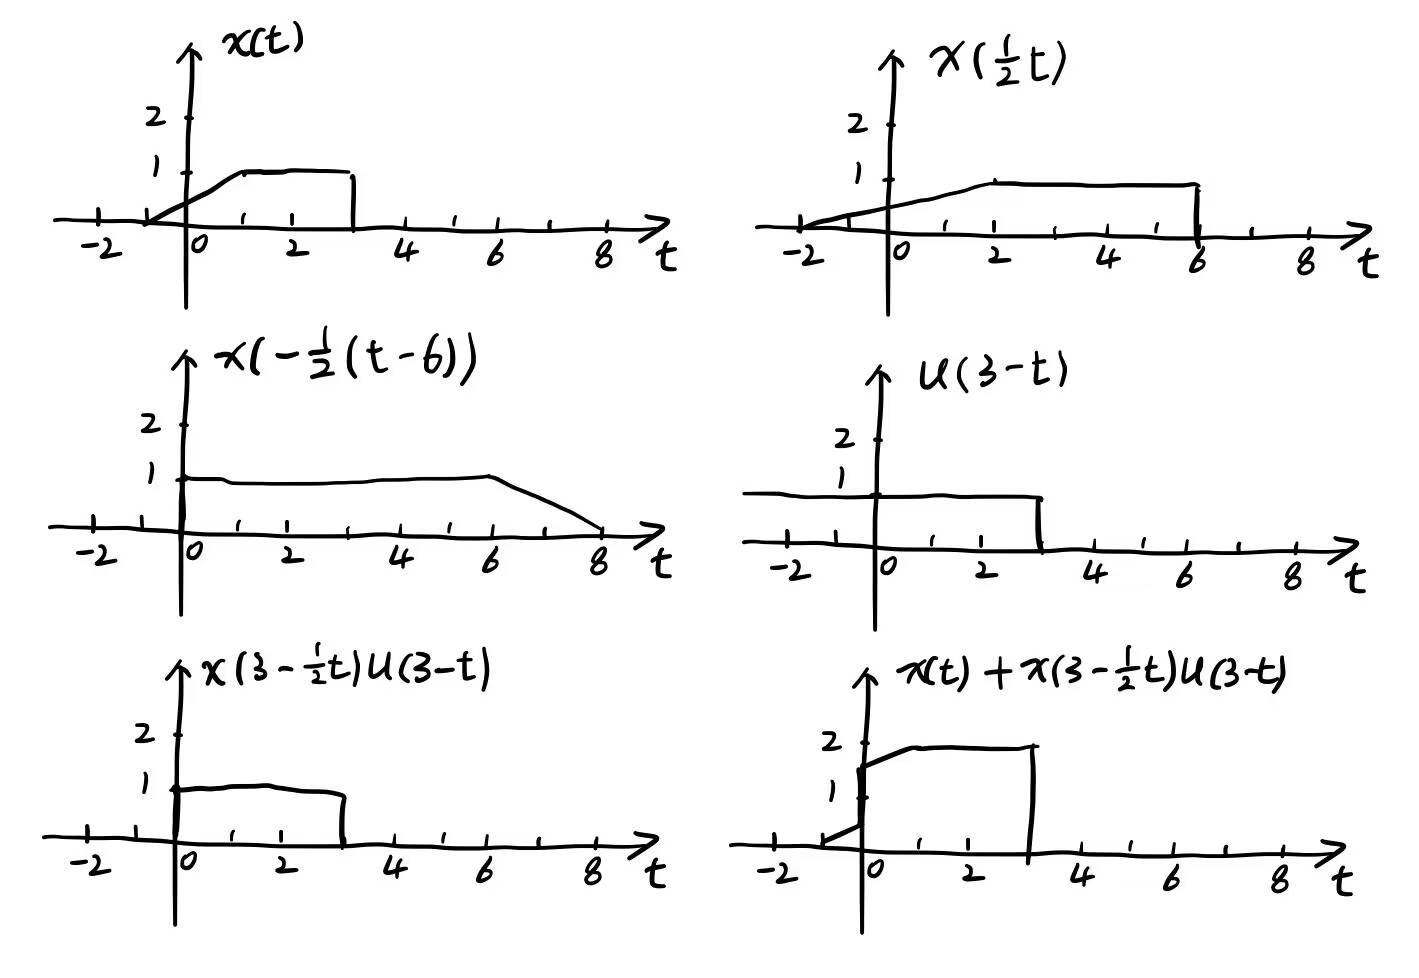
\includegraphics[width=0.9\textwidth]{images/2022-11-17-16-22-51.png}
        \label{Fig.main1}
      \end{figure}
      
      最后的图像为右下角所示, 表达式为:
      
      $\displaystyle x(t) + x(3-\frac{1}{2}t)u(3-t) = \begin{cases}
      \frac{1}{2}(t+1), & t \in [-1, 0] \\
      \frac{1}{2}(t+3), & t \in [0, 1] \\
      2, & t \in [1, 3] \\
      0, & \text{otherwise}
      \end{cases}$
      
      \item (2)
      
      $\displaystyle x'(t) = -\delta(t-3) + y(t)$, 其中 $y(t) = \begin{cases}
      \frac{1}{2}, & t \in [-1, 1] \\
      0, & \text{otherwise}
      \end{cases}$
      
      $\displaystyle x''(t) = \frac{1}{2}\delta(t+1) - \frac{1}{2}\delta(t-1) - \delta'(t-3)$
      
      因此有
      
      $\displaystyle x'(t) - x''(t) = y(t) - \frac{1}{2}\delta(t+1) + \frac{1}{2}\delta(t-1) - \delta(t-3) + \delta'(t-3)$
      
      图像为:

      \begin{figure}[H]
        \centering
        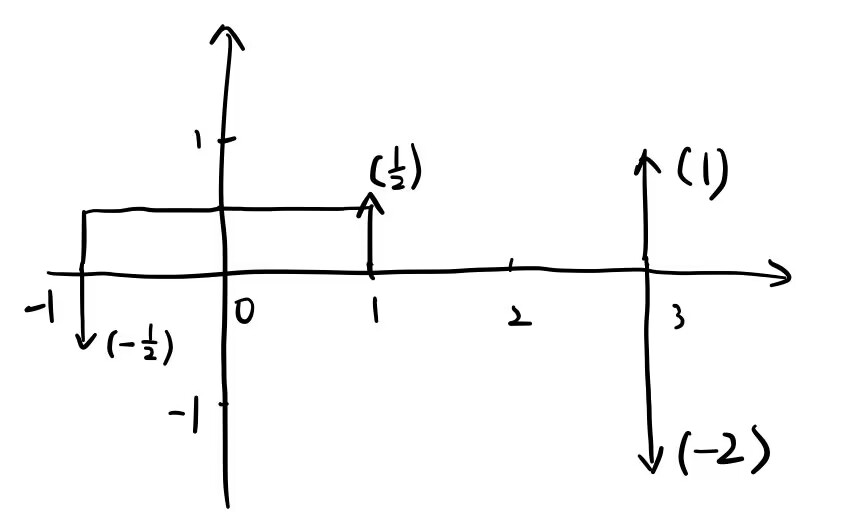
\includegraphics[width=0.9\textwidth]{images/2022-11-18-10-11-58.png}
        \label{Fig.main1}
      \end{figure}
      

      \item (3)
      
      由于 $x(t)$ 只在 $t \in [-1, 3]$ 处有正值, 其他情况下 $x(t) = 0$, 因此有 $x(t), x(t+4n), x(t-4n), n=1,2,\cdots, \infty$ 互不冲突, 即任取 $t \in (-\infty, \infty)$ 都仅有其中一个函数值非零. 
      
      展开 $h(t)$ 即可得
      
      $
      \begin{aligned}
      h(t) &= \sum_{n = 0}^{\infty}\frac{1}{2^{n}}[x(t+4n)+x(t-4n)] \\
      &= 2x(t) + \sum_{n = 1}^{\infty}\frac{1}{2^{n}}[x(t+4n)+x(t-4n)] \\
      &=\begin{cases}
      t+1, & t \in [-1, 1] \\
      2, & t \in [1, 3] \\
      \frac{1}{2^{n+1}}[(t \mp 4n)+1], & t \in [-1 \pm 4n, 1 \pm 4n], n = 1, 2, \cdots, \infty \\
      \frac{1}{2^{n}}, & t \in [1 \pm 4n, 3 \pm 4n], n = 1, 2, \cdots, \infty \\
      \end{cases} \\
      \end{aligned}
      $
      
      能量:
      
      $
      \begin{aligned}
      W &= \lim_{T \to \infty}\int_{-T}^{T}|h(t)|^{2}\mathrm{d}t \\
      &= \int_{-1}^{1}(t+1)^{2}\mathrm{d}t + \int_{-1}^{1}2^{2}\mathrm{d}t + 2\sum_{n=1}^{\infty}\int_{-1+4n}^{1+4n}(\frac{1}{2^{n+1}}[(t - 4n)+1])^{2}\mathrm{d}t  \\
      &\quad\ + 2\sum_{n=1}^{\infty}\int_{1+4n}^{3+4n}(\frac{1}{2^{n}})^{2}\mathrm{d}t \\
      &= \frac{8}{3} + 8 + 2\sum_{n=1}^{\infty}\int_{-1}^{1}(\frac{t+1}{2^{n+1}})^{2}\mathrm{d}t + 2\sum_{n=1}^{\infty}\int_{1}^{3}(\frac{1}{2^{n}})^{2}\mathrm{d}t \\
      &= \frac{8}{3} + 8 + 2\sum_{n=1}^{\infty}\frac{1}{2^{2n+2}}\cdot \frac{8}{3} + 2\sum_{n=1}^{\infty}\frac{1}{2^{2n}}\cdot 2 \\
      &= \frac{8}{3} + 8 + \frac{4}{9} + \frac{4}{3} \\
      &= \frac{112}{9} \\
      \end{aligned}
      $
      
      功率: $\displaystyle P = \lim_{T \to \infty}\frac{1}{2T}W = 0$
      
      因此可知 $h(t)$ 是能量信号.
    \end{itemize}
\end{spacing}
\end{framed}


\newpage
\section{[28pts] 卷积的计算 }
计算下列各小题的结果:
\begin{enumerate}[(1)]
	\item 设
	\begin{equation*}
        \begin{aligned}
        x(t)=\left\{
        \begin{aligned}
        & 2t+1, && t\in[-1,1]\\
        & 3, && t\in[1,3]\\
        & 0, && other
        \end{aligned}
        \right.
        \end{aligned}
    \end{equation*}
    试求$x(t)*x(t)$的结果。
	\item 求$y(t)=[2e^{-2(t-1)}u(t-2)]*[3e^{-3(t+1)}u(t-1)]$的表达式。
	\item 设$x(n)=\{1,1,4,5,1,4\}$, $y(n)=\{1,9,1,9,8,1\}$, 求$x(n)*y(n)$.
	\item 设
	\begin{equation*}
        \begin{aligned}
        x(n)=\left\{
        \begin{aligned}
        & n, && n=1,2,...k\\
        & 0, && other
        \end{aligned}
        \right.
        \end{aligned}
    \end{equation*}
    试求$x(n)*x(n)$的结果。
\end{enumerate}

\begin{framed}
\begin{spacing}{1.5}
    \begin{itemize}
      \item (1)

      当 $t < -2$ 时, 有 $\displaystyle x(t) * x(t) = \int_{-\infty}^{\infty}x(\tau)x(t-\tau)\mathrm{d}\tau = 0$

      当 $-2 \le t < 0$ 时, 
      
      $
      \begin{aligned}
      x(t) * x(t) &= \int_{-\infty}^{\infty}x(\tau)x(t-\tau)\mathrm{d}\tau  \\
      &= \int_{-1}^{t+1}(2\tau+1)(2(t-\tau)+1)\mathrm{d}\tau  \\
      &= \int_{-1}^{t+1}(- 4 \tau^{2} + 4 t \tau + 2 t + 1)\mathrm{d}\tau  \\
      &= (- \frac{4}{3} \tau^{3} + 2 t \tau^{2} + (2 t + 1)\tau)|_{-1}^{t+1}  \\
      &= (- \frac{4}{3} (t+1)^{3} + 2 t (t+1)^{2} + (2 t + 1)(t+1)) \\
      &\quad\ - (- \frac{4}{3} (-1)^{3} + 2 t (-1)^{2} + (2 t + 1)(-1))  \\
      &= \frac{2 t^{3}}{3} + 2 t^{2} + t - \frac{2}{3}  \\
      \end{aligned}
      $
      
      当 $0 \le t < 2$ 时,
      
      $
      \begin{aligned}
      x(t) * x(t) &= \int_{-\infty}^{\infty}x(\tau)x(t-\tau)\mathrm{d}\tau  \\
      &= \int_{-1}^{t-1}3(2\tau+1)\mathrm{d}\tau + \int_{t-1}^{1}(2\tau+1)(2(t-\tau)+1)\mathrm{d}\tau \\
      &\quad\ + \int_{1}^{t+1}3(2(t-\tau)+1)\mathrm{d}\tau  \\
      &= 3(\tau^{2}+\tau)|_{-1}^{t-1} + (- \frac{4}{3} \tau^{3} + 2 t \tau^{2} + (2 t + 1)\tau)|_{t-1}^{1} \\
      &\quad\ + 3(-\tau^{2} + (2 t+1)\tau)|_{1}^{t+1}  \\
      &= 3t (t - 1) + (- \frac{2 t^{3}}{3} - 2 t^{2} + 7 t - \frac{2}{3}) + 3t (t - 1) \\
      &= - \frac{2 t^{3}}{3} + 4 t^{2} + t - \frac{2}{3} \\
      \end{aligned}
      $
      
      当 $2 \le t < 4$ 时,
      
      $
      \begin{aligned}
      x(t) * x(t) &= \int_{-\infty}^{\infty}x(\tau)x(t-\tau)\mathrm{d}\tau  \\
      &= \int_{t-3}^{1}3(2\tau+1)\mathrm{d}\tau + \int_{1}^{t-1}9\mathrm{d}\tau + \int_{t-1}^{3}3(2(t-\tau)+1)\mathrm{d}\tau  \\
      &= 3(\tau^{2}+\tau)|_{t-3}^{1} + 9\tau|_{1}^{t-1} + 3(-\tau^{2} + (2 t+1)\tau)|_{t-1}^{3}  \\
      &= - 6 t^{2} + 39 t - 42  \\
      \end{aligned}
      $
      
      当 $4 \le t < 6$ 时,
      
      $
      \begin{aligned}
      x(t) * x(t) &= \int_{-\infty}^{\infty}x(\tau)x(t-\tau)\mathrm{d}\tau  \\
      &= \int_{t-3}^{3}9\mathrm{d}\tau  \\
      &= 54 - 9 t  \\
      \end{aligned}
      $
      
      当 $t \ge 6$ 时, $\displaystyle x(t) * x(t) = \int_{-\infty}^{\infty}x(\tau)x(t-\tau)\mathrm{d}\tau = 0$
      
      因此我们有
      
      $x(t) * x(t) = \begin{cases}
          0, & t < -2 \\
          \frac{2 t^{3}}{3} + 2 t^{2} + t - \frac{2}{3}, & -2 \le t < 0  \\
          - \frac{2 t^{3}}{3} + 4 t^{2} + t - \frac{2}{3}, & 0 \le t < 2 \\
          - 6 t^{2} + 39 t - 42, & 2 \le t < 4 \\
          54 - 9 t, & 4 \le t < 6 \\
          0, & t \ge 6 \\
      \end{cases}$
      
      \item (2)
      
      当 $t < 3$ 时, $y(t) = 0$
      
      当 $t \ge 3$ 时,
      
      $
      \begin{aligned}
      y(t) &= [2e^{-2(t-1)}u(t-2)] * [3e^{-3(t+1)}u(t-1)] \\
      &= \int_{2}^{t-1}[2e^{-2(\tau-1)}]\cdot [3e^{-3(t-\tau+1)}]\mathrm{d}\tau \\
      &= \int_{2}^{t-1}6 e^{\tau - 3 t  - 1}\mathrm{d}\tau \\
      &= 6 e^{\tau - 3 t  - 1}|_{2}^{t-1} \\
      &= 6 e^{- 2 t - 2} - 6 e^{1 - 3 t} \\
      \end{aligned}
      $
      
      因此有
      
      $y(t) = \begin{cases}
          6 e^{- 2 t - 2} - 6 e^{1 - 3 t}, & t \ge 3 \\
          0, & t < 3 \\
      \end{cases}$
      
      \item (3)
      
      当 $n = 0$ 时, $x(n) * y(n) = 1 \times 1 = 1$
      
      当 $n = 1$ 时, $x(n) * y(n) = 1 \times 9 + 1 \times 1 = 10$
      
      当 $n = 2$ 时, $x(n) * y(n) = 1 \times 1 + 1 \times 9 + 4 \times 1 = 14$
      
      当 $n = 3$ 时, $x(n) * y(n) = 1 \times 9 + 1 \times 1 + 4 \times 9 + 5 \times 1 = 51$
      
      当 $n = 4$ 时, $x(n) * y(n) = 1 \times 8 + 1 \times 9 + 4 \times 1 + 5 \times 9 + 1 \times 1 = 67$
      
      当 $n = 5$ 时, $x(n) * y(n) = 1 \times 1 + 1 \times 8 + 4 \times 9 + 5 \times 1 + 1 \times 9 + 4 \times 1 = 63$
      
      当 $n = 6$ 时, $x(n) * y(n) = 1 \times 1 + 4 \times 8 + 5 \times 9 + 1 \times 1 + 4 \times 9 = 115$
      
      当 $n = 7$ 时, $x(n) * y(n) = 4 \times 1 + 5 \times 8 + 1 \times 9 + 4 \times 1 = 57$
      
      当 $n = 8$ 时, $x(n) * y(n) = 5 \times 1 + 1 \times 8 + 4 \times 9 = 49$
      
      当 $n = 9$ 时, $x(n) * y(n) = 1 \times 1 + 4 \times 8 = 33$
      
      当 $n = 10$ 时, $x(n) * y(n) = 4 \times 1 = 4$
      
      因此有 $x(n) * y(n) = \{ 1, 10, 14, 51, 67, 63, 115, 57, 49, 33, 4 \}$
      
      \item (4)
      
      $x(n)$ 也可以改写为
      
      $x(n) = \begin{cases}
          n, & n = 0, 1, 2, \cdots, k \\
          0, & \text{otherwise}
      \end{cases}$
      
      当 $0 \le n \le k$ 时,
      
      $\displaystyle x(n) * x(n) = \sum_{i=0}^{n}x(i)x(n-i) = \sum_{i=0}^{n}i(n-i) = \frac{1}{6}n (n^{2} - 1)$
      
      当 $k+1 \le n \le 2k+1$ 时,
      
      $
      \begin{aligned}
      x(n) * x(n) & = \sum_{i=n-k}^{k}x(i)x(n-i)  \\
      & = \sum_{i=n-k}^{k}i(n-i)  \\
      & = n\sum_{i=n-k}^{k}i-\sum_{i=n-k}^{k}i^{2}  \\
      & = n\cdot \frac{n (2 k - n + 1)}{2}-(\frac{n(n+1)(2n+1)}{6})|_{n-k-1}^{k}  \\
      & = - \frac{1}{6}(2 k - n + 1) (2 k^{2} - 2 k n + 2 k - n^{2} - n) \\
      \end{aligned}
      $
      
      因此可得
      
      $x(n) * x(n) = \begin{cases}
        \frac{1}{6}n (n^{2} - 1), & 0 \le n \le k \\
        - \frac{1}{6}(2 k - n + 1) (2 k^{2} - 2 k n + 2 k - n^{2} - n), & k+1 \le n \le 2k+1 \\
        0, & \text{otherwise}
      \end{cases}$
      
      此处的 $x(n) * x(n)$ 依然是从 0 开始的, 而非从 1 开始的.
    \end{itemize}
\end{spacing}
\end{framed}


\newpage
\section{[30pts] 系统微分方程的求解 }
求解以下微分方程:
\begin{enumerate}[(1)]
	\item $y^{(2)}(t)+7y^{(1)}(t)+12y(t)=2\sin(2t)$ $(t\geqslant0)$, 边界条件$y(0)=0,y^{(1)}(0)=1$.
	\item $y(n)-\displaystyle\frac{3}{4}y(n-1)+\frac{1}{16}y(n-3)=x(n)-x(n-1)$ $(n\geqslant0)$,其中$x(n)=\displaystyle\left(\frac{1}{3}\right)^n$,边界条件$y(0)=y(1)=0,y(2)=1$。
\end{enumerate}

\begin{framed}
\begin{spacing}{1.5}
    \begin{itemize}
      \item (1)

      求齐次解, 特征方程为

      $\alpha^{2}+7\alpha+12 = (\alpha + 3) (\alpha + 4) = 0$
      
      齐次解为 $y_h(t) = A_1 e^{-3t} + A_2 e^{-4t}$
      
      求特解, 设特解形式为 $y_p(t) = B_1 \cos(2t) + B_2 \sin(2t)$
      
      带入可得
      
      $
      \begin{aligned}
      & \quad\ y_p^{(2)}(t) + 7y_p^{(1)}(t) + 12y_p(t)  \\
      & = - 4 B_{1} \cos(2t) - 4 B_{2} \sin(2t) - 14B_1\sin(2t) + 14B_2\cos(2t)  \\
      &\quad\ + 12B_1 \cos(2t) + 12B_2 \sin(2t)  \\
      & = (8 B_{1} + 14 B_{2})\cos(2 t) + (- 14 B_{1} + 8 B_{2}) \sin(2 t)  \\
      & = 2\sin(2 t)  \\
      \end{aligned}
      $
      
      因此有 $\begin{cases}
          8 B_{1} + 14 B_{2} = 0 \\
          - 14 B_{1} + 8 B_{2} = 2 \\
      \end{cases}$ 即有 $\begin{cases}
          B_{1} = - \frac{7}{65} \\
          B_{2} = \frac{4}{65} \\
      \end{cases}$
      
      因此我们有
      
      $\displaystyle y(t) = y_h(t) + y_p(t) = A_1 e^{-3t} + A_2 e^{-4t} - \frac{7}{65}\cos(2t) + \frac{4}{65}\sin(2t)$
      
      根据初始条件有
      
      $
      \begin{cases}
          \displaystyle y(0) = A_{1} + A_{2} - \frac{7}{65} = 0  \\
          \displaystyle y^{(1)}(0) = - 3 A_{1} - 4 A_{2} + \frac{8}{65}= 1  \\
      \end{cases}
      $
      
      解得 $\displaystyle A_{1} = \frac{17}{13}, A_{2} = - \frac{6}{5}$
      
      因此有 $\displaystyle y(t) = y_h(t) + y_p(t) = \frac{17}{13} e^{-3t} + - \frac{6}{5} e^{-4t} - \frac{7}{65}\cos(2t) + \frac{4}{65}\sin(2t)$
      
      \item (2)
      
      求齐次解, 特征方程为 $\displaystyle \alpha^{3}-\frac{3}{4}\alpha^{2}+\frac{1}{16} = \frac{1}{16}(4 \alpha + 1)(2 \alpha - 1)^{2} = 0$
      
      特征根为 $\displaystyle \alpha_1 = -\frac{1}{4}, \alpha_2 = \alpha_3 = \frac{1}{2}$
      
      齐次解为 $\displaystyle y_h(n) = A_1 (-\frac{1}{4})^{n} + (A_2 + A_3n)(\frac{1}{2})^{n}$
      
      设特解为 $\displaystyle y_p(n) = C(\frac{1}{3})^{n}$
      
      带入可得
      
      $
      \begin{aligned}
      &\quad\ y_p(n) - \frac{3}{4}y_p(n-1) + \frac{1}{16}y_p(n-3) \\
      &= C(\frac{1}{3})^{n} - \frac{3}{4}C(\frac{1}{3})^{n-1} + \frac{1}{16}C(\frac{1}{3})^{n-3} \\
      &= \frac{7}{16}C(\frac{1}{3})^{n} \\
      &= x(n) - x(n-1) \\
      &= (\frac{1}{3})^{n} - (\frac{1}{3})^{n-1} \\
      &= - 2 \cdot (\frac{1}{3})^{n} \\
      \end{aligned}
      $
      
      因此可得 $\displaystyle C = -2 \times \frac{16}{7} = - \frac{32}{7}$
      
      特解为: $\displaystyle y_p(n) = - \frac{32}{7}\cdot (\frac{1}{3})^{n}$
      
      因此我们有
      
      $\displaystyle y(n) = y_h(n) + y_p(n) = A_1 (-\frac{1}{4})^{n} + (A_2 + A_3n)(\frac{1}{2})^{n} - \frac{32}{7}\cdot (\frac{1}{3})^{n}$
      
      我们带入初始条件得
      
      $
      \begin{cases}
          \displaystyle y(0) = A_{1} + A_{2} - \frac{32}{7} = 0 \\
          \displaystyle y(1) = - \frac{A_{1}}{4} + \frac{A_{2}}{2} + \frac{A_{3}}{2} - \frac{32}{21} = 0 \\
          \displaystyle y(2) = \frac{A_{1}}{16} + \frac{A_{2}}{4} + \frac{A_{3}}{2} - \frac{32}{63} = 1 \\
      \end{cases}
      $
      
      解得
      
      $
      \begin{cases}
          A_{1} = \frac{1136}{567} \\
          A_{2} = \frac{208}{81} \\
          A_{3} = \frac{40}{27} \\
      \end{cases}
      $
      
      因此有
      
      $\displaystyle y(n) = \frac{1136}{567} (-\frac{1}{4})^{n} + (\frac{208}{81} + \frac{40}{27}n)(\frac{1}{2})^{n} - \frac{32}{7}\cdot (\frac{1}{3})^{n}$
    \end{itemize}
\end{spacing}
\end{framed}


\newpage
\end{document}